%!TEX root = Thesis_main.tex

\chapter{Experiments Setup}
\label{chapter6}

The Mobile Manipulator under analisys in this thesis is a prototype assembled at University of Southern California in the Center of Advance Manufacturing (CAM) Laboratory. The system has been called ADDAMS: A*********** and is shown in figure \ref{imgADDAMS.png}. (IMMAGINE TEMPORANEA)

\begin{figure}[h] \label{imgADDAMS1}
	\begin{center} 
		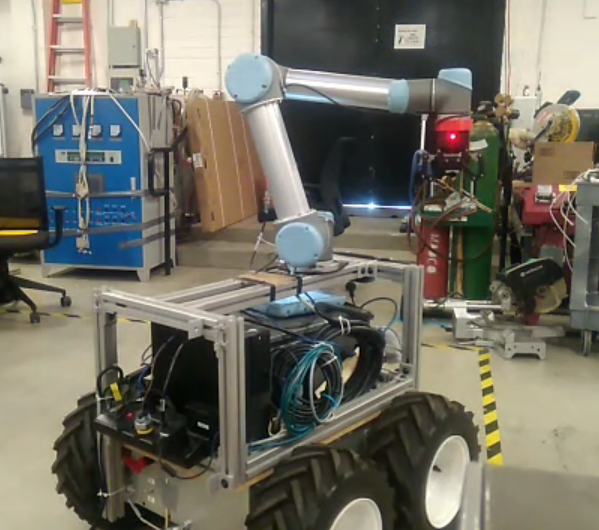
\includegraphics[scale=0.4]{imgADDAMS.png}
		\centering
	\end{center}
\end{figure}

 The goal of this prototype is to study a system able to handle parts as well as to perform operations in unstructured industrial enviroments to fill the gap between small and large production systems. Indeed, companies with small production volumes are nowdays required to innovate production systems towards the generation of smart factories. Given that those companies are generally not economically able to manage automated production lines and that the production mix is generally changed frequently, flexible systems to support production are required. For those reasons ADDAMS wants to be a low cost solution, using low cost sensors and to be capable, once it's operation have been planned, to perform in any enviroment. \\

The controller presented in this thesis wants to be the first step towards the design of an online software that make the system able to operate autonomously once the task has been given. In the next sections the main components of ADDAMS will be shown in its Hardare and Software parts then, setups used for simulations and physical tests will be presented. 



\section{Hardware}

\subsection{Mobile Base}

\begin{figure}[h]
	\begin{center} 
		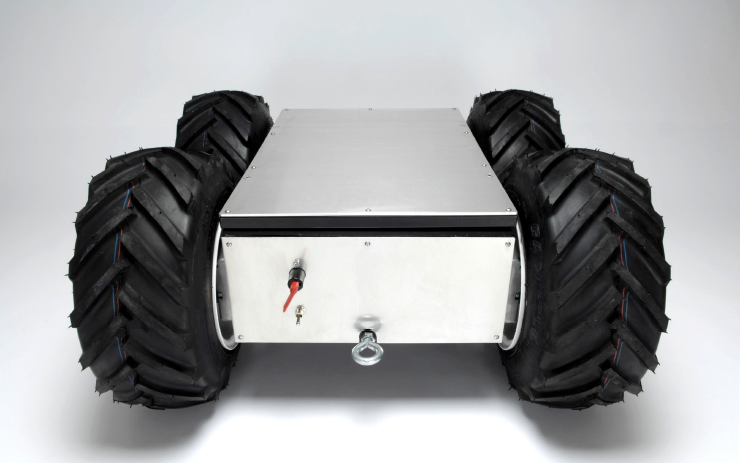
\includegraphics[scale=0.6]{SuperMegaBot1}
		\centering
		\caption{Nonholomic Mobile base}
		\label{fig:SuperMegaBot1}
	\end{center}
\end{figure}
The mobile base, provided by InspectorBots and named Super Mega Bot, is a Heavy-Duty, All-Terrain, 4WD robotic platform shown in figure \ref{fig:SuperMegaBot1}. It is a rugged, Indoor/outdoor, remotely operated platform and can be fitted with a variety of sensors, cameras and equipment. The base has been designed to be Modular and Reconfigurable, so an end user can swap out various modules. There are several methods available to control the SMB provided by the manufacturer including: RC radio, Analog Joystick, Wireless Modem, or Microcomputer.\\
The SMB is designed with non-steering coupled wheels and because of that the rotation of the base is obtained giving different velocities to the right and left wheels. For this reason the SMB is configured as a differential drive mobile robot for which the kinematic relationships explained in \ref{chapter2} hold.
In appendix \ref{appA} can be found technical data of the SMB and informations about the motor used.

\subsection{UR5 Manipulator}
The UR5 is a collaborative robotic arm developed by Universal Robots. According to the company the key benefits of their robots are that they are light weight, safe and easy to use. The robotic arm is regarded as safe, because it will stop acting as soon as the robot hits an object sensed by a force sensor in one of the joints. UR5 is ideal for automating low-weight processing tasks like picking, placing and testing. The medium-sized robot arm is easy to program, fast to set up and, always according to UR, offers one of the fastest payback times in the industry. Because it is designed as a collobarative robot, the UR5 is generally suitable for tasks in which the operative space of the robot is shared with humans and that fits also ADDAMS objectives. The UR5 comes from the manufacturer with its control unit that can be easily accessed and provide low level controllers for tracking velocities of the joints. More technincal details on UR5 can be found in appendix \ref{appB}.

\begin{figure}[htbp]
	\begin{center} 
		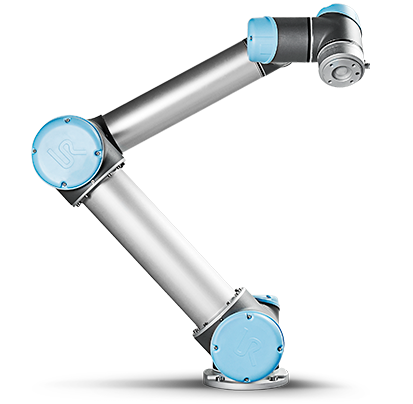
\includegraphics[scale=0.4]{UR5}
		\centering
		\label{fig:UR5} 
	\end{center}
\end{figure}


\subsection{Sensors}

The sensors of the ADDAMS prototype will be used to measure positions of the joints to perform the desired task. Breafly the sensor system is composed of:
\begin{itemize}
	\item Anglular encoders for the UR5 joints wich provide an accuracy of $0.1$ mm
	\item Encoders on the wheels of the base that will be used to derive the position and orientation of the mobile base through a simple transformation. This measuring system is reliable only at slow speed and provide an accuracy of $\pm 2$ cm. Because the position of the end effector is computed knowing the position of the base, the accuracy of this measures is not sufficient to perform precise operation. Considerations on this aspect will be done later on.
	\item Lidar that can be used to measure unknown obstacles position in the operative area of the robot.
	(AGGIUNGERE ANCHE LE TELECAMERE? OPPURE LE METTIAMO DA QUALCHE PARTE FACENDO UNA CONSIDERAZIONE SULLA SENSORISTICA?)
\end{itemize}

\section{Software}

To easily interface with all the components of ADDAMS we used ROS, an open-source, meta-operating system for robotic systems. ROS provides the services that allow communication between all the components, message-passing between processes, hardware abstraction, low-level device control. It also provides tools and libraries for obtaining, building, writing, and running code across multiple computers. The ROS network used to run the Phisical system is shown in the graph \ref{ROSnodes}

\begin{figure}[htbp]
	\begin{center} 
		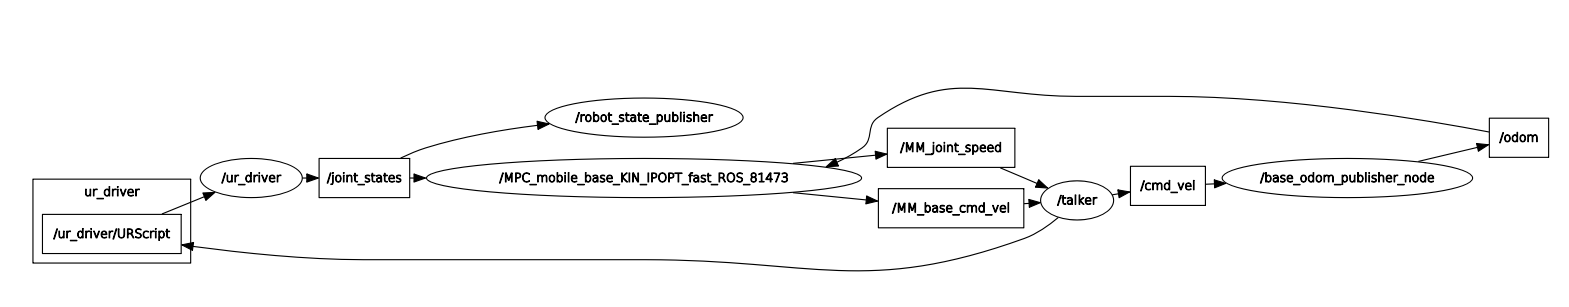
\includegraphics[scale=0.24]{nodegraph2}
		\centering
		\label{ROSnodes} 
		\caption{ROS nodes and messages for ADDAMS}
	\end{center}
\end{figure}

The controller we designed has been developed using Matlab/Simulink enviroment through the CasADi, an open-source tool for nonlinear optimization and algorithmic differentiation that allows using Matlab/Simulink to define optimization problems and different commercial solvers. More information about CasADi can be found in \cite{Andersson2018}. The solver used to solve the Nonlinear Problem defined in \ref{chapter5} is IPOPT, a brief introduction to IPOPT can be found in Appendix \ref{appC}. As shown in graph \ref{ROSnodes} the simulink node where the controller is running reads position of the base and joint angles and give velocity commands to the system through a "talker" node we defined to communicate with the robot. As already mentioned the commands given to the system are velocity commands, i.e. high level commands that the system is required to track. Anyway, given that the manufacturers already provides reliable low level controllers able to track those desired velocities, we decided to use, as mentioned in \ref{chapter5}, a hierarchical approach that is breafly explained in figure \ref{Hdiagram}.  
\begin{figure}[h!]
	\begin{center} 
		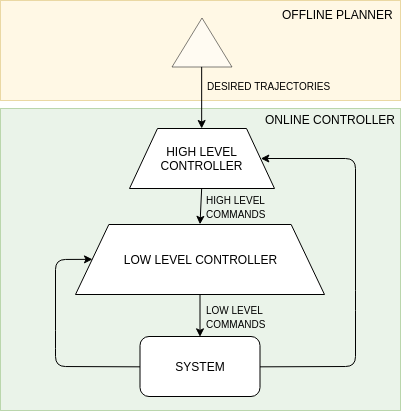
\includegraphics[scale=0.35]{Hdiagram}
		\centering
		\label{Hdiagram}
		\caption{Control hierarchy} 
	\end{center}
\end{figure}
\\
Simulations and Physical experiments have been carried out to test the developed controller and to analyze performances and influences of parameters. In particular two conditions have been tested: 

\begin{itemize}
	\item \textbf{Movement of the system toward grasping area}. Referring to the controller as presented in \ref{chapter5} we will consider the cost function \ref{costfunctionh} as a composition of $h_4$ and $h_5$. In fact the task of moving the system towards grasping area is performed controllig the base position and the joint angles positions without requiring to track end effector position. The choice of this formulation for the cost function allows the problem to be easier to solve given that we are tracking joint angles rather than EE position, computed through forward Kinematics. Futhermore, the arm is generally not required to move during the movement of the system outside grasping areas.

	\item \textbf{Trajectory tracking inside graping area}. In this case, as already mentioned, we will consider the problem of tracking the EE position considering the cost function \ref{costfunctionh} as a composition of $h_1$, $h_2$ and $h_3$. This task is more of interest of this thesis and then will be discussed more in detail than the first one. Considerations about online changing the cost function will be given in the next section. 

\section{Simulations setup}

	Simulations for both the tasks object of study have been performed using Simulink to test stability, robustness, performances and effects of the parameters on the controller. The model used to simulate the system is basically the same presented in \ref{chapter2} that has been numerically integrated to allows calculating positions. The block diagram in figure \ref{simdiagram1} shows the simple achitecture of the controller used in simulations.

	\begin{figure}[h!]
	\begin{center} 
		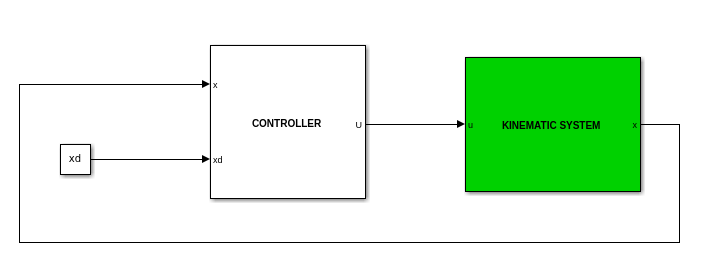
\includegraphics[scale=0.35]{simdiagram1}
		\centering
		\label{simdiagram1}
		\caption{Simulations block diagram} 
	\end{center}
	\end{figure}

	The results of the simulations have been saved and processed in MATLAB R2018b. The frequency used  
	
	
\section{Phisical Experiments Setup}
	
	block diagram esperimenti reali simulink

	low lwvwl controllers and considerations
